\documentclass[tikz,border=8pt]{standalone}
\usepackage{lmodern}\usetikzlibrary{arrows.meta,positioning,fit,backgrounds}
\definecolor{aws}{HTML}{EAF2F8}\definecolor{optional}{HTML}{FFF1DE}\tikzset{box/.style={draw,rounded corners,fill=aws,minimum width=28mm,minimum height=11mm,align=center,font=\sffamily\scriptsize},opt/.style={box,fill=optional},client/.style={box,fill=black!5},external/.style={box,fill=black!8},edge/.style={-{Latex[length=1.7mm]},thick,font=\sffamily\tiny,align=center},async/.style={edge,dashed}}
\begin{document}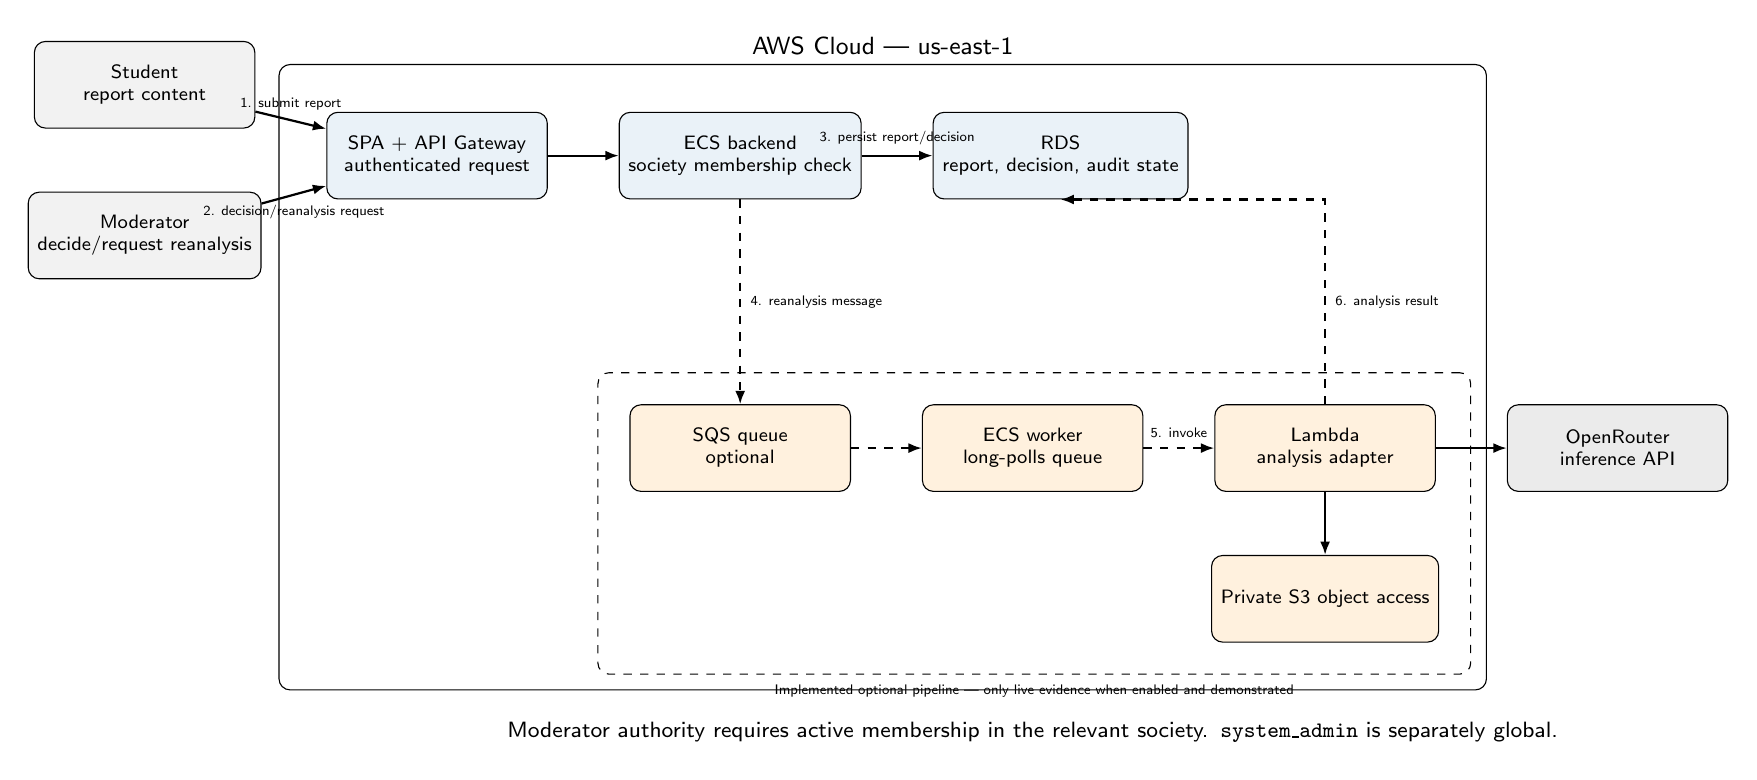
\begin{tikzpicture}[node distance=8mm and 9mm]
\node[client] (student) {Student\\report content};\node[client,below=of student] (moderator) {Moderator\\decide/request reanalysis};\node[box,right=of student,yshift=-9mm] (spa) {SPA + API Gateway\\authenticated request};\node[box,right=of spa] (ecs) {ECS backend\\society membership check};\node[box,right=of ecs] (rds) {RDS\\report, decision, audit state};
\node[opt,below=26mm of ecs] (sqs) {SQS queue\\optional};\node[opt,right=of sqs] (worker) {ECS worker\\long-polls queue};\node[opt,right=of worker] (lambda) {Lambda\\analysis adapter};\node[opt,below=of lambda] (s3) {Private S3 object access};\node[external,right=of lambda] (openrouter) {OpenRouter\\inference API};
\draw[edge] (student) -- node[above]{1. submit report} (spa);\draw[edge] (moderator) -- node[below]{2. decision/reanalysis request} (spa);\draw[edge] (spa) -- (ecs);\draw[edge] (ecs) -- node[above]{3. persist report/decision} (rds);
\draw[async] (ecs) -- node[right]{4. reanalysis message} (sqs);\draw[async] (sqs) -- (worker);\draw[async] (worker) -- node[above]{5. invoke} (lambda);\draw[edge] (lambda) -- (openrouter);\draw[edge] (lambda) -- (s3);\draw[async] (lambda) |- node[pos=.25,right]{6. analysis result} (rds.south);
\begin{scope}[on background layer]\node[draw,rounded corners,fit=(spa)(ecs)(rds)(sqs)(worker)(lambda)(s3),inner sep=6mm,label={[font=\sffamily\small]above:AWS Cloud --- us-east-1}] {};\node[draw,dashed,rounded corners,fit=(sqs)(worker)(lambda)(s3),inner sep=4mm,label={[font=\sffamily\tiny]below:Implemented optional pipeline --- only live evidence when enabled and demonstrated}] {};\end{scope}
\node[font=\sffamily\footnotesize,align=center,text width=150mm,below=28mm of worker] {Moderator authority requires active membership in the relevant society. \texttt{system\_admin} is separately global.};
\end{tikzpicture}\end{document}
